\documentclass[a4paper]{jsarticle}
\usepackage[dvipdfmx]{graphicx}
\usepackage{amsmath}
\usepackage{bm}
\renewcommand{\thesection}{第\arabic{section}問}
\renewcommand{\thesubsection}{(\arabic{subsection})}
\renewcommand{\thesubsubsection}{(\alph{subsubsection})}
\begin{document}

\title{2016分野3}
\author{nakao}
\maketitle

\section{}
\subsection{}
\subsubsection{}
管路に作用する力を右向き正で$f$とすると、流体には$-f$の力が作用する。
断面$\mathrm{I}$,$\mathrm{I}\hspace{-1.2pt}\mathrm{I}$での流速をそれぞれ$v_1, v_2$、
断面$\mathrm{I}\hspace{-1.2pt}\mathrm{I}$(噴射直前)における圧力を$p_2$とすると、
運動量保存則から
\begin{equation}
  \rho Q v_2 - \rho Q v_1 = -f + p_1 A_1 - p_2 \frac{A_1}{4}
\end{equation}
が成り立つ。
ここで連続式
$Q = A_1 v_1 = \frac{A_1}{4} v_2$より、
\begin{align}
  v_1 &= \frac{Q}{A_1} \\
  v_2 &= \frac{4Q}{A_1}
\end{align}
である。また、Bernoulliの定理
\begin{equation}
  \frac{v_1^2}{2g} + \frac{p_1}{\rho g}
  = \frac{v_2^2}{2g} + \frac{p_2}{\rho g}
\end{equation}
より、
\begin{equation}
  p_2 = p_1 - \frac{\rho}{2} (v_2^2 - v_1^2)
  = p_1 - \frac{15 \rho Q^2}{2 A_1^2}
\end{equation}
である。式(2),(3),(5)を式(1)に代入すると、
\begin{equation}
  f = \frac{3 p_1 A_1}{4} - \frac{9 \rho Q^2}{8 A_1}
\end{equation}
を得る。

\subsubsection{}
断面$\mathrm{I}\hspace{-1.2pt}\mathrm{I}$(噴射直前)と
板に衝突した後の流れで運動量保存を考え、
\begin{equation}
  -\rho Q v_2 = -F + p_2 \frac{A_1}{4}
\end{equation}
が成り立つ。式(3),(5)をこれに代入して、
\begin{equation}
  F = \frac{p_1 A_1}{4} + \frac{17 \rho Q^2}{8 A_1}
\end{equation}
を得る。

\subsection{}
\subsubsection{}
容器から観測すると$-2g$の物体力が鉛直方向に作用する。水圧分布は図1のようになる。
\subsubsection{}
容器から観測すると物体力が作用しない。水圧分布は図2のようになる。
\begin{figure}[htb]
  \begin{minipage}{0.4\hsize}
    \centering
    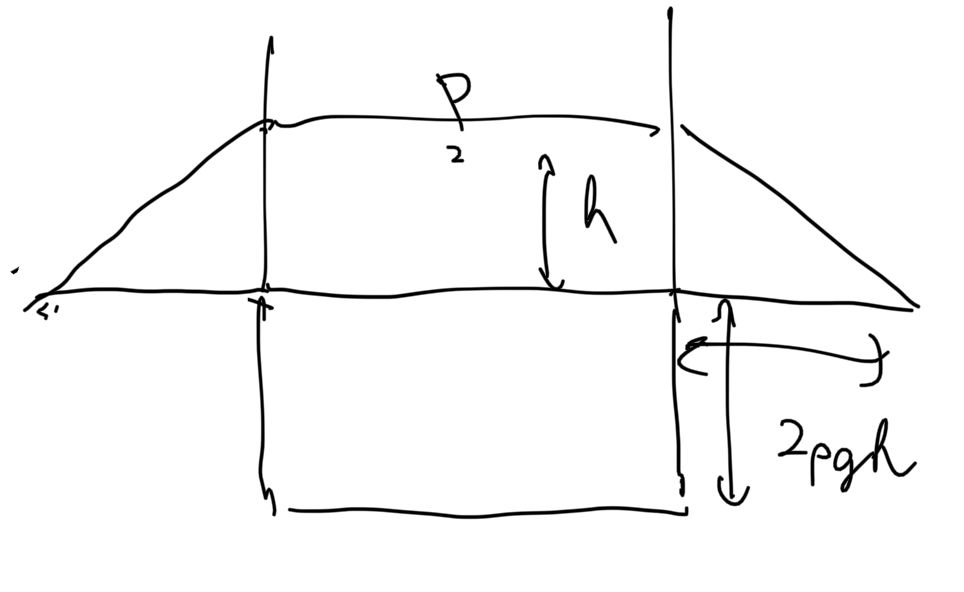
\includegraphics[width=\hsize]{fig1.png}
    \caption{(a)の水圧分布}
  \end{minipage}
  \begin{minipage}{0.4\hsize}
    \centering
    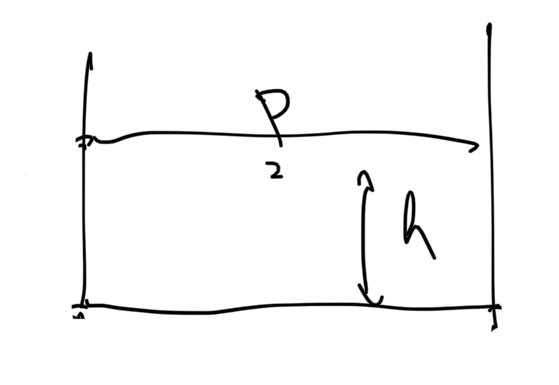
\includegraphics[width=0.5\hsize]{fig2.png}
    \caption{(b)の水圧分布}
  \end{minipage}
\end{figure}

\subsection{}
鉛直方向の運動方程式は、
\begin{equation}
  \frac{\partial w}{\partial t}
  + u \frac{\partial w}{\partial x}
  + w \frac{\partial w}{\partial z}
  = - \frac{1}{\rho} \frac{\partial p}{\partial z} - g
\end{equation}
である。壁面付近では鉛直方向の流速が卓越し$u \ll w$であるとして、式(9)は
\begin{equation}
  \frac{\partial w}{\partial t}
  + w \frac{\partial w}{\partial z}
  = - \frac{1}{\rho} \frac{\partial p}{\partial z} - g
\end{equation}
で近似でき、これより
\begin{equation}
  \frac{\partial p}{\partial z} = -\rho g
  - \rho \left(\frac{\partial w}{\partial t}
  + w \frac{\partial w}{\partial z}\right)
\end{equation}
を得る。\par
点Aの水圧を$p_A$として、問題文の図5の状態の壁面における水面高さを$h$とする。
このとき、
\begin{equation}
  \int_0^h \frac{\partial p}{\partial z} \mathrm{d} z = 0 - p_A
\end{equation}
であるから、
\begin{equation}
  p_A = -\int_0^h \frac{\partial p}{\partial z} \mathrm{d} z
\end{equation}
と表せる。これに式(11)を代入すると、
\begin{equation}
  p_A = \int_0^h \left\{\rho g
  + \rho \left(\frac{\partial w}{\partial t}
  + w \frac{\partial w}{\partial z}\right)\right\} \mathrm{d} z
  = \rho g h + \rho \int_0^h
  \left(\frac{\partial w}{\partial t}
  + w \frac{\partial w}{\partial z}\right) \mathrm{d} z
\end{equation}
を得る。問題の図5の流速分布では$0 \leq z \leq h$で
$\frac{\partial w}{\partial t} > 0, \frac{\partial w}{\partial z} > 0$
であり、$p_A > \rho g h$となっている。

\section{}
\subsection{}
連続式$q = v_1 C_c h_1 = v_0 h_0$より
$v_0 = C_c h_1 v_1 / h_0$であり、これをベルヌーイの定理
\begin{equation}
  \frac{v_0^2}{2g} + h_0 = \frac{v_1^2}{2g} + C_c h_1
\end{equation}
に代入すると、
\begin{equation}
  v_1 = h_0 \sqrt{\frac{2g}{h_0 + C_c h_1}}
\end{equation}
を得る。したがって、
\begin{equation}
  q = v_1 C_c h_1 = C_c h_0 h_1 \sqrt{\frac{2g}{h_0 + C_c h_1}}
\end{equation}
である。\par
ゲート開口部では渦運動が卓越しているため、流量算出においてはA地点の水深を用いる必要がある。

\subsection{}
運動量保存則から
\begin{equation}
  \rho q v_3 - \rho q v_2 = \frac{1}{2} \rho g h_2^2 - \frac{1}{2} \rho g h_3^2
\end{equation}
が成り立つ。連続式より
$v_2 = q / h_2, v_3 = q / h_3$であり、これを代入すると、
\begin{equation}
  h_2 = \frac{1}{2} \left(\sqrt{h_3^2 + \frac{8 q^2}{g h_3}} - h_3\right)
\end{equation}
を得る。

\subsection{}
式(19)を$h_2$で微分すると、
\begin{equation}
  \frac{\partial h_2}{\partial h_3} =
  \frac{1}{2} \left(\frac{2h_3 - \frac{8q^2}{g h_3^2}}{2 \sqrt{h_3^2 + \frac{8q^2}{gh_3}}} - 1\right) =
  \frac{1}{4 \sqrt{h_3^2 + \frac{8q^2}{gh_3}}} \left(2h_3 - 2 \sqrt{h_3^2 + \frac{8q^2}{gh_3}} - \frac{8q^2}{gh_3^2}\right) < 0
\end{equation}
であるから、$h_3$の増加に対して、$h_2$は減少する。\par
A地点で跳水が起こるためには、$h_2 = C_c h_1$であればよい。
このとき式(19)より、
\begin{equation}
  \frac{1}{2} \left(\sqrt{h_3^2 + \frac{8 q^2}{g h_3}} - h_3\right) = C_c h_1
\end{equation}
であり、ここに式(17)を代入して$h_3$について解くと、
\begin{equation}
  h_3 = \frac{1}{2} \left(\sqrt{C_c^2 h_1^2 + \frac{16 C_c h_0^2 h_1}{h_0 + C_c h_1}} - C_c h_1\right)
\end{equation}
を得る。
\subsection{}
副ダムが高すぎる場合は、ダムのかなり手前のエネルギーが大きい状態で跳水が起こる。
副ダムが低すぎる場合は、跳水が起こらない。
\end{document}